\documentclass[14pt,a4paper]{article}
\usepackage[utf8]{inputenc}
\usepackage[T1]{fontenc}
\usepackage{lmodern}
\usepackage{geometry}
\geometry{margin=1.5cm}
\usepackage{graphicx}
\usepackage{hyperref}
\usepackage{listings}
\usepackage{xcolor}
\usepackage{enumitem}
\usepackage{float}
\usepackage{booktabs}
\usepackage{titlesec}
\usepackage{titling}
\usepackage{fancyhdr}
\usepackage{tcolorbox}
\usepackage{tikz}
\usepackage{pgf-umlcd}
\usepackage{mdframed}
\usepackage{array}
\usepackage{tabularx}
\usepackage{caption}
\usepackage{subcaption}

% Enhanced typography
\usepackage{setspace}
\onehalfspacing

% Header and footer setup
\pagestyle{fancy}
\fancyhf{}
\fancyhead[L]{\slshape Court Kart: E-Commerce Platform}
\fancyhead[R]{\slshape \thepage}
\fancyfoot[C]{\small HADJ ARAB Adel - E-Commerce Project}
\renewcommand{\headrulewidth}{0.4pt}
\renewcommand{\footrulewidth}{0.4pt}

% Title formatting
\pretitle{\begin{center}\LARGE\bfseries}
\posttitle{\par\end{center}\vspace{0.5em}}
\preauthor{\begin{center}\large}
\postauthor{\end{center}}
\predate{\begin{center}\large}
\postdate{\end{center}\vspace{1em}}

% Section formatting
\titleformat{\section}
  {\normalfont\large\bfseries\color[RGB]{0,83,138}}
  {\thesection}{1em}{}[\titlerule]
\titlespacing*{\section}
  {0pt}{3.5ex plus 1ex minus .2ex}{2.3ex plus .2ex}

\titleformat{\subsection}
  {\normalfont\normalsize\bfseries\color[RGB]{70,130,180}}
  {\thesubsection}{1em}{}
\titlespacing*{\subsection}
  {0pt}{3.25ex plus 1ex minus .2ex}{1.5ex plus .2ex}

% Define code listing style
\definecolor{codegreen}{rgb}{0,0.6,0}
\definecolor{codegray}{rgb}{0.5,0.5,0.5}
\definecolor{codepurple}{rgb}{0.58,0,0.82}
\definecolor{backcolour}{rgb}{0.95,0.95,0.95}
\definecolor{customblue}{RGB}{0,83,138}

\lstdefinestyle{mystyle}{
    backgroundcolor=\color{backcolour},   
    commentstyle=\color{codegreen},
    keywordstyle=\color{blue},
    stringstyle=\color{codepurple},
    basicstyle=\ttfamily\footnotesize,
    breakatwhitespace=false,         
    breaklines=true,                 
    captionpos=b,                    
    keepspaces=true,                 
    numbers=left,                    
    numbersep=5pt,                  
    showspaces=false,                
    showstringspaces=false,
    showtabs=false,                  
    tabsize=2,
    frame=single,
    framexleftmargin=5pt,
    framextopmargin=5pt,
    framexbottommargin=5pt
}

\lstset{style=mystyle}

% Custom box environments
\newtcolorbox{infobox}{
  colback=blue!5!white,
  colframe=blue!75!black,
  coltext=black,
  boxrule=0.5mm,
  arc=4pt,
  title=Note
}

% Hyperref setup for better PDF metadata and navigation
\hypersetup{
    colorlinks=true,
    linkcolor=blue,
    filecolor=magenta,
    urlcolor=customblue,
    pdftitle={Court Kart: E-Commerce Platform Design Document},
    pdfauthor={HADJ ARAB Adel},
    pdfsubject={E-Commerce Platform},
    pdfkeywords={e-commerce, database, triggers, stored procedures, PHP, MySQL},
    pdfcreator={LaTeX},
    pdfproducer={pdfLaTeX}
}

\title{\textbf{Court Kart: E-Commerce Platform}\\[0.5em]\Large Design and Implementation Document}
\author{\textbf{HADJ ARAB Adel}}
\date{\today}

\begin{document}

\maketitle

\begin{abstract}
	\noindent This document presents the design and implementation of Court Kart, an e-commerce platform specializing in basketball equipment and apparel. The system is built using PHP, MySQL, and JavaScript, following the Model-View-Controller (MVC) architectural pattern. Key features include user authentication, product management, shopping cart functionality, order processing, and an administrative interface. The database implementation leverages advanced MySQL features including stored procedures and triggers to ensure data integrity and business rule enforcement. This document provides comprehensive details about the system architecture, database design, and implementation of required features.
\end{abstract}

\newpage
\tableofcontents
\newpage

\section{Introduction}

Court Kart is a comprehensive e-commerce platform specializing in sports equipment and apparel, with a primary focus on basketball products. The application follows modern web development patterns with a clean separation of concerns, using PHP for server-side processing, MySQL for database management, and JavaScript for client-side interactivity.

\subsection{Project Overview}
The Court Kart platform facilitates online shopping for basketball enthusiasts, offering features such as product browsing, detailed product views, user account management, shopping cart functionality, and secure checkout process. The platform also includes an administrative interface for managing products, orders, and users.

\subsection{Technologies Used}
The platform is built using the following technologies:
\begin{itemize}
	\item \textbf{Backend:} PHP 8.1 with custom MVC framework
	\item \textbf{Database:} MySQL 8.0
	\item \textbf{Frontend:} HTML5, CSS3, JavaScript (ES6+)
	\item \textbf{Version Control:} Git
	\item \textbf{Additional Libraries:} Font Awesome for icons
\end{itemize}

\begin{figure}[H]
	\centering
	% \includegraphics[width=0.9\textwidth]{images/technologies_stack.png}
	\caption{Technology Stack Architecture}
	\label{fig:tech-stack}
\end{figure}

\section{System Architecture}

\subsection{Architectural Pattern}
Court Kart implements the Model-View-Controller (MVC) architectural pattern to ensure separation of concerns and maintainability:

\begin{itemize}
	\item \textbf{Model:} Handles data logic and database interactions, encapsulating business rules and data access
	\item \textbf{View:} Renders the user interface using PHP templates with embedded HTML and CSS
	\item \textbf{Controller:} Processes user input, coordinates data flow between Model and View components
	\item \textbf{Core Components:} Provides fundamental functionality like routing, database connections, session management, and security
\end{itemize}

\begin{figure}[H]
	\centering
	% \includegraphics[width=0.8\textwidth]{images/mvc_architecture.png}
	\caption{Model-View-Controller Architecture Diagram}
	\label{fig:mvc}
\end{figure}

\subsection{Directory Structure}
The application follows a well-organized directory structure that separates different concerns:

\begin{figure}[H]
	\centering
	% \includegraphics[width=0.9\textwidth]{images/directory_structure.png}
	\caption{Project Directory Structure}
	\label{fig:directory}
\end{figure}

\begin{lstlisting}[caption={Detailed Directory Structure}, label={lst:directory}]
/court-kart-store
  /config           # Application configuration files
    database.php    # Database connection settings
    app.php         # Application settings
  /src              # Application source code
    /Controllers    # Request handlers
    /Models         # Data models and business logic
    /Core           # Framework components
      Router.php    # URL routing system
      Database.php  # Database connection and query builder
      View.php      # Template rendering engine
      Session.php   # Session management
      Middleware.php # Request filtering
    /Services       # Business logic services
    /Helpers        # Utility functions
  /views            # UI templates
    /layouts        # Page templates and partials
    /shop           # Shop-related views
    /cart           # Shopping cart views
    /checkout       # Checkout process views
    /admin          # Admin interface views
    /auth           # Authentication views
    /errors         # Error pages
  /public           # Publicly accessible files
    /assets         # Static resources
      /css          # Stylesheets
      /js           # JavaScript files
      /images       # Image files
      /fonts        # Font files
  /routes           # Route definitions
    web.php         # Web routes
  /sql              # Database schema and scripts
    schema.sql      # Database tables
    triggers.sql    # Database triggers
    procedures.sql  # Stored procedures
  /docs             # Documentation files
    report.tex      # This design document
    images/         # Documentation images
\end{lstlisting}

\subsection{Request Lifecycle}
The following sequence diagram illustrates the lifecycle of a typical request in the Court Kart application:

\begin{figure}[H]
	\centering
	% \includegraphics[width=0.95\textwidth]{images/request_lifecycle.png}
	\caption{Request Lifecycle Sequence Diagram}
\end{figure}

\section{Database Design}

\subsection{Entity-Relationship Diagram}
The database schema is designed to support all e-commerce functionality while maintaining data integrity and relational constraints:

\begin{figure}[H]
	\centering
	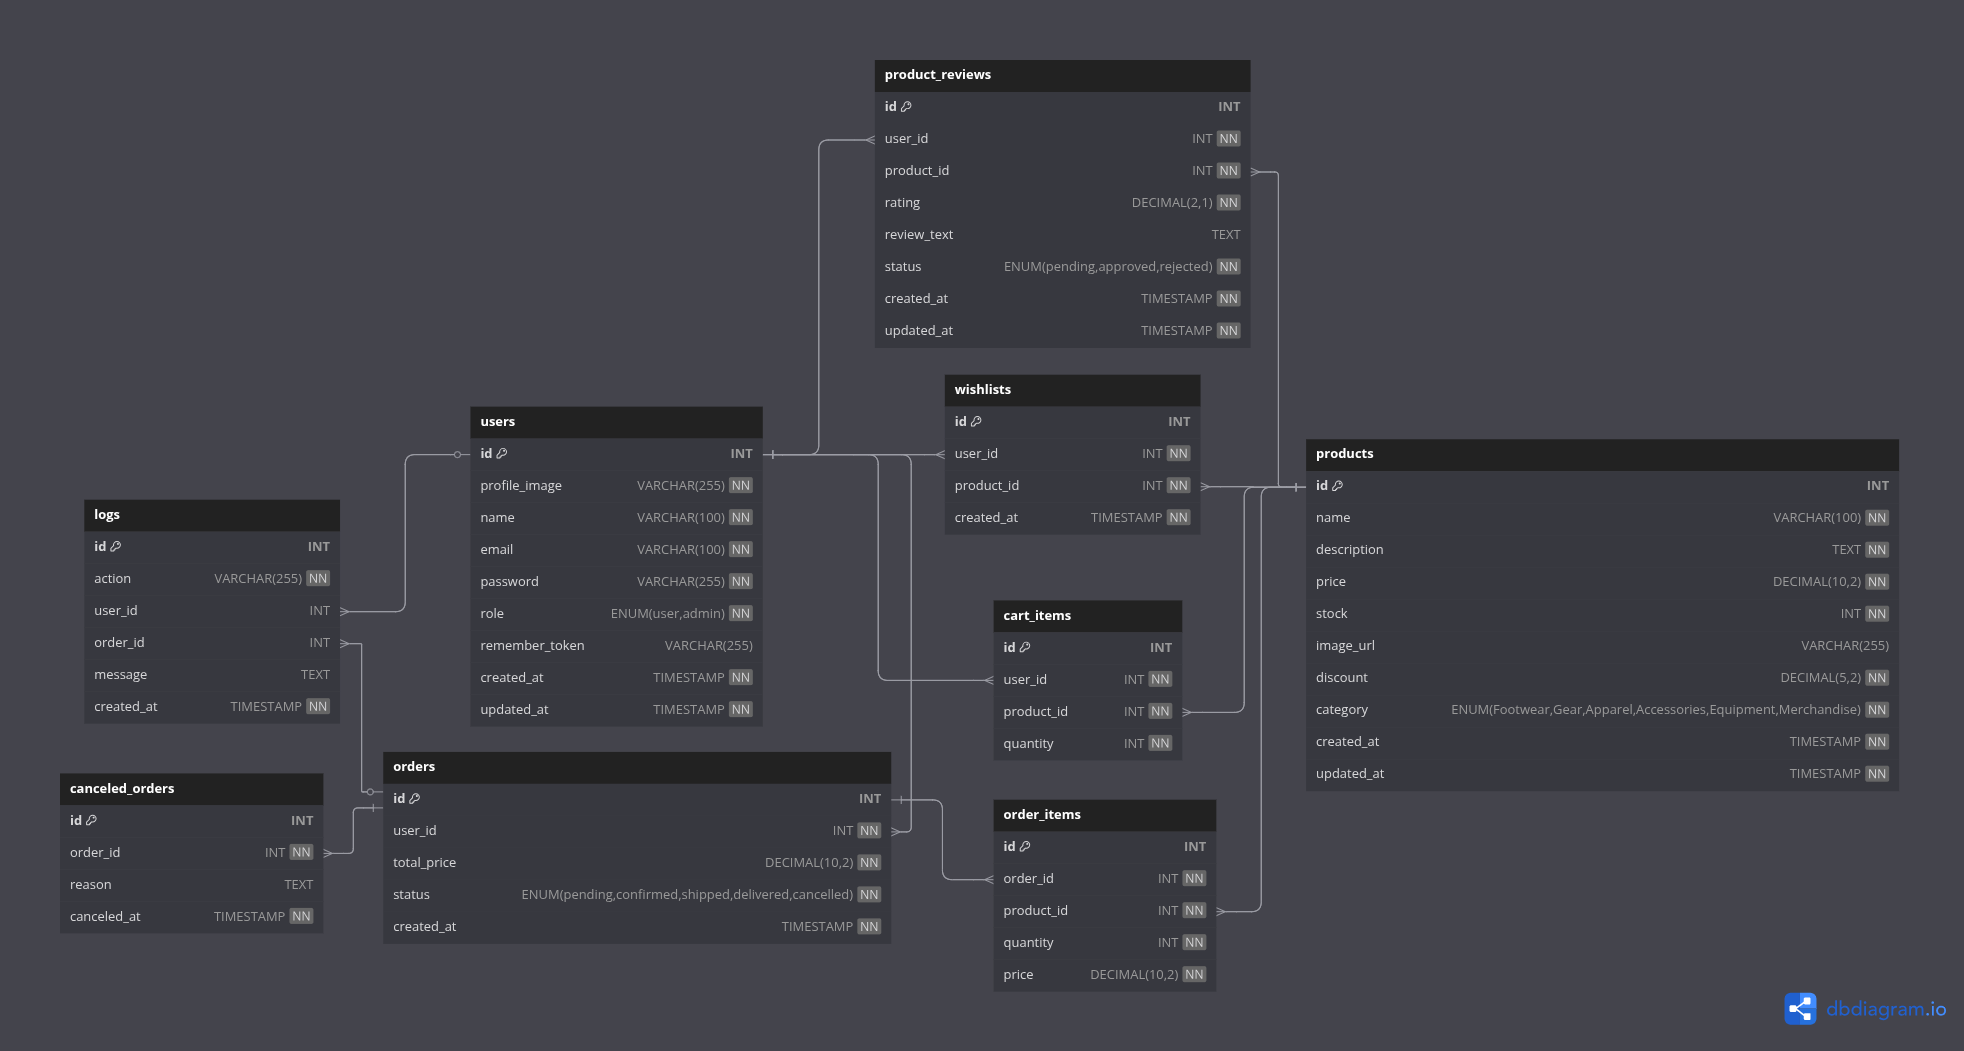
\includegraphics[width=1\textwidth]{../public/assets/images/db-schema.png}
	\caption{Entity-Relationship Diagram}
\end{figure}

\subsection{Database Schema}
Court Kart's database consists of several interconnected tables designed to support all e-commerce functionality:

\begin{table}[H]
	\centering
	\caption{Database Schema Overview}
	\label{tab:schema}
	\begin{tabularx}{\textwidth}{|l|l|X|}
		\hline
		\textbf{Table Name} & \textbf{Primary Key} & \textbf{Description}                                                                                                         \\
		\hline
		users               & id (INT)             & Stores user account information including authentication data, profile details, and role designation (admin or regular user) \\
		\hline
		products            & id (INT)             & Contains comprehensive product details including name, description, pricing, stock levels, category, and image references    \\
		\hline
		categories          & id (INT)             & Stores product categories for hierarchical organization of the product catalog                                               \\
		\hline
		cart\_items         & id (INT)             & Links users to products in their shopping cart with quantity information                                                     \\
		\hline
		orders              & id (INT)             & Maintains order headers with status tracking, user references, and timestamps                                                \\
		\hline
		order\_items        & id (INT)             & Contains line items associated with each order, including product information, quantity, and price at time of purchase       \\
		\hline
		canceled\_orders    & id (INT)             & Records canceled orders with reason information and timestamps for business analytics                                        \\
		\hline
		logs                & id (INT)             & Comprehensive system activity tracking for auditing and debugging purposes                                                   \\
		\hline
	\end{tabularx}
\end{table}

\subsection{Table Relationships}
The database implements the following relationships to maintain data integrity:

\begin{itemize}
	\item \textbf{users $\rightarrow$ cart\_items:} One-to-many (A user can have multiple items in their cart)
	\item \textbf{users $\rightarrow$ orders:} One-to-many (A user can place multiple orders)
	\item \textbf{products $\rightarrow$ cart\_items:} One-to-many (A product can be in multiple users' carts)
	\item \textbf{products $\rightarrow$ order\_items:} One-to-many (A product can be in multiple orders)
	\item \textbf{orders $\rightarrow$ order\_items:} One-to-many (An order contains multiple products)
	\item \textbf{orders $\rightarrow$ canceled\_orders:} One-to-one (A canceled order references exactly one order)
	\item \textbf{categories $\rightarrow$ products:} One-to-many (A category contains multiple products)
\end{itemize}

\subsection{Detailed Table Specifications}

\begin{mdframed}[backgroundcolor=blue!5, linecolor=blue!40, linewidth=1pt]
	\textbf{users}
	\begin{lstlisting}[language=SQL, numbers=none]
CREATE TABLE users (
    id INT PRIMARY KEY AUTO_INCREMENT,
    name VARCHAR(100) NOT NULL,
    email VARCHAR(255) NOT NULL UNIQUE,
    password VARCHAR(255) NOT NULL,
    role ENUM('user', 'admin') DEFAULT 'user',
    profile_image VARCHAR(255) NULL,
    remember_token VARCHAR(100) NULL,
    created_at TIMESTAMP DEFAULT CURRENT_TIMESTAMP,
    updated_at TIMESTAMP DEFAULT CURRENT_TIMESTAMP ON UPDATE CURRENT_TIMESTAMP
);
\end{lstlisting}
\end{mdframed}

\begin{mdframed}[backgroundcolor=blue!5, linecolor=blue!40, linewidth=1pt]
	\textbf{products}
	\begin{lstlisting}[language=SQL, numbers=none]
CREATE TABLE products (
    id INT PRIMARY KEY AUTO_INCREMENT,
    name VARCHAR(255) NOT NULL,
    description TEXT NOT NULL,
    price DECIMAL(10,2) NOT NULL,
    stock INT NOT NULL DEFAULT 0,
    category VARCHAR(50) NOT NULL,
    image_url VARCHAR(255) NOT NULL,
    is_new BOOLEAN DEFAULT FALSE,
    discount INT DEFAULT 0,
    created_at TIMESTAMP DEFAULT CURRENT_TIMESTAMP,
    updated_at TIMESTAMP DEFAULT CURRENT_TIMESTAMP ON UPDATE CURRENT_TIMESTAMP
);
\end{lstlisting}
\end{mdframed}

\begin{mdframed}[backgroundcolor=blue!5, linecolor=blue!40, linewidth=1pt]
	\textbf{orders}
	\begin{lstlisting}[language=SQL, numbers=none]
CREATE TABLE orders (
    id INT PRIMARY KEY AUTO_INCREMENT,
    user_id INT NOT NULL,
    total_price DECIMAL(10,2) NOT NULL,
    status ENUM('pending', 'confirmed', 'shipped', 'delivered', 'cancelled') DEFAULT 'pending',
    created_at TIMESTAMP DEFAULT CURRENT_TIMESTAMP,
    updated_at TIMESTAMP DEFAULT CURRENT_TIMESTAMP ON UPDATE CURRENT_TIMESTAMP,
    FOREIGN KEY (user_id) REFERENCES users(id) ON DELETE CASCADE
);
\end{lstlisting}
\end{mdframed}

\begin{mdframed}[backgroundcolor=blue!5, linecolor=blue!40, linewidth=1pt]
	\textbf{order\_items}
	\begin{lstlisting}[language=SQL, numbers=none]
CREATE TABLE order_items (
    id INT PRIMARY KEY AUTO_INCREMENT,
    order_id INT NOT NULL,
    product_id INT NOT NULL,
    quantity INT NOT NULL,
    price DECIMAL(10,2) NOT NULL,
    FOREIGN KEY (order_id) REFERENCES orders(id) ON DELETE CASCADE,
    FOREIGN KEY (product_id) REFERENCES products(id) ON DELETE NO ACTION
);
\end{lstlisting}
\end{mdframed}

\section{Stored Procedures Implementation}

The database includes several stored procedures to handle complex business logic directly at the database level. This approach enhances performance, reduces network traffic, and centralizes business rule enforcement.

\subsection{GetOrderDetails}

This stored procedure retrieves comprehensive information about a specific order, including all ordered items, product details, and pricing information.

\begin{lstlisting}[language=SQL, caption={GetOrderDetails Stored Procedure}, label={lst:get-order-details}]
DELIMITER $$

CREATE PROCEDURE GetOrderDetails(IN p_order_id INT)
BEGIN
    -- Get order items with product details
    SELECT 
        oi.order_id,
        oi.product_id,
        p.name AS product_name,
        oi.quantity,
        oi.price AS unit_price,
        (oi.quantity * oi.price) AS subtotal,
        p.image_url
    FROM 
        order_items oi
    JOIN 
        products p ON oi.product_id = p.id
    WHERE 
        oi.order_id = p_order_id;
END$$

DELIMITER ;
\end{lstlisting}

\textbf{Usage Example:}
\begin{lstlisting}[language=SQL, numbers=none]
CALL GetOrderDetails(123);
\end{lstlisting}

\subsection{FinalizeOrder}

This stored procedure handles the checkout process by confirming the order and removing items from the customer's cart.

\begin{lstlisting}[language=SQL, caption={FinalizeOrder Stored Procedure}, label={lst:finalize-order}]
DELIMITER $$

CREATE PROCEDURE FinalizeOrder(IN p_order_id INT, IN p_user_id INT)
BEGIN
    DECLARE v_order_exists INT;
    
    -- Start transaction to ensure atomicity
    START TRANSACTION;
    
    -- Check if order exists and belongs to the user
    SELECT COUNT(*) INTO v_order_exists 
    FROM orders 
    WHERE id = p_order_id AND user_id = p_user_id;
    
    IF v_order_exists = 0 THEN
        SIGNAL SQLSTATE '45000' 
        SET MESSAGE_TEXT = 'Order not found or does not belong to this user';
        ROLLBACK;
    ELSE
        -- Update order status to 'confirmed'
        UPDATE orders 
        SET status = 'confirmed' 
        WHERE id = p_order_id;
        
        -- Clear cart items for this user
        DELETE FROM cart_items 
        WHERE user_id = p_user_id;
        
        -- Log the order finalization
        INSERT INTO logs (action, user_id, order_id, message) 
        VALUES ('ORDER_FINALIZED', p_user_id, p_order_id, CONCAT('Order #', p_order_id, ' has been finalized'));
        
        COMMIT;
    END IF;
END$$

DELIMITER ;
\end{lstlisting}

\textbf{Usage Example:}
\begin{lstlisting}[language=SQL, numbers=none]
CALL FinalizeOrder(123, 456);
\end{lstlisting}

\subsection{GetCustomerOrderHistory}

This stored procedure retrieves a customer's complete order history with detailed information.

\begin{lstlisting}[language=SQL, caption={GetCustomerOrderHistory Stored Procedure}, label={lst:customer-order-history}]
DELIMITER $$

CREATE PROCEDURE GetCustomerOrderHistory(IN p_user_id INT)
BEGIN
    -- Get all orders for the user with item counts
    SELECT 
        o.id AS order_id,
        o.created_at,
        o.total_price AS total,
        o.status,
        COUNT(oi.id) AS items_count,
        GROUP_CONCAT(p.name SEPARATOR ', ') AS product_names
    FROM 
        orders o
    LEFT JOIN 
        order_items oi ON o.id = oi.order_id
    LEFT JOIN 
        products p ON oi.product_id = p.id
    WHERE 
        o.user_id = p_user_id
    GROUP BY 
        o.id
    ORDER BY 
        o.created_at DESC;
END$$

DELIMITER ;
\end{lstlisting}

\textbf{Usage Example:}
\begin{lstlisting}[language=SQL, numbers=none]
CALL GetCustomerOrderHistory(456);
\end{lstlisting}

\section{Database Triggers Implementation}

Triggers are used to enforce business rules and maintain data integrity automatically when certain database events occur.

\subsection{AfterOrderConfirmed}

This trigger automatically updates product stock quantities when an order status changes to "confirmed".

\begin{lstlisting}[language=SQL, caption={AfterOrderConfirmed Trigger}, label={lst:after-order-confirmed}]
DELIMITER $$

CREATE TRIGGER AfterOrderConfirmed
AFTER UPDATE ON orders
FOR EACH ROW
BEGIN
    DECLARE v_done INT DEFAULT 0;
    DECLARE v_product_id INT;
    DECLARE v_quantity INT;
    DECLARE cur CURSOR FOR 
        SELECT product_id, quantity FROM order_items WHERE order_id = NEW.id;
    DECLARE CONTINUE HANDLER FOR NOT FOUND SET v_done = 1;

    IF OLD.status != 'confirmed' AND NEW.status = 'confirmed' THEN
        -- Log the order confirmation
        INSERT INTO logs (action, user_id, order_id, message)
        VALUES ('CHECKOUT', NEW.user_id, NEW.id, CONCAT('Order #', NEW.id, ' confirmed'));

        -- Update product stock for each item in the order
        OPEN cur;
        read_loop: LOOP
            FETCH cur INTO v_product_id, v_quantity;
            IF v_done THEN
                LEAVE read_loop;
            END IF;
            
            -- Decrease product stock
            UPDATE products
            SET stock = stock - v_quantity
            WHERE id = v_product_id;
        END LOOP;
        CLOSE cur;
        
        -- Log stock updates
        INSERT INTO logs (action, user_id, order_id, message)
        VALUES ('PRODUCT_UPDATE', NEW.user_id, NEW.id, CONCAT('Stock updated for order #', NEW.id));
    END IF;
END$$

DELIMITER ;
\end{lstlisting}

\subsection{BeforeOrderItemInsert}

This trigger prevents adding products to orders if the requested quantity exceeds available stock.

\begin{lstlisting}[language=SQL, caption={BeforeOrderItemInsert Trigger}, label={lst:before-order-item-insert}]
DELIMITER $$

CREATE TRIGGER BeforeOrderItemInsert
BEFORE INSERT ON order_items
FOR EACH ROW
BEGIN
    DECLARE available_stock INT;
    DECLARE v_user_id INT;
    
    -- Get available stock for the product
    SELECT stock INTO available_stock
    FROM products
    WHERE id = NEW.product_id;
    
    -- Get user ID for logging
    SELECT user_id INTO v_user_id
    FROM orders
    WHERE id = NEW.order_id;

    -- Check if we have enough stock
    IF NEW.quantity > available_stock THEN
        -- Log the stock violation attempt
        INSERT INTO logs (action, user_id, order_id, message)
        VALUES ('PRODUCT_UPDATE', v_user_id, NEW.order_id, 
                CONCAT('Failed to add product #', NEW.product_id, ' to order #', NEW.order_id, 
                       ': Requested ', NEW.quantity, ', Available ', available_stock));
                
        -- Raise an error to prevent the insert
        SIGNAL SQLSTATE '45000'
        SET MESSAGE_TEXT = 'Cannot insert order item: requested quantity exceeds available stock';
    END IF;
END$$

DELIMITER ;
\end{lstlisting}

\subsection{AfterOrderCancelled}

This trigger restores product stock quantities when an order is canceled.

\begin{lstlisting}[language=SQL, caption={AfterOrderCancelled Trigger}, label={lst:after-order-cancelled}]
DELIMITER $$

CREATE TRIGGER AfterOrderCancelled
AFTER UPDATE ON orders
FOR EACH ROW
BEGIN
    DECLARE v_done INT DEFAULT 0;
    DECLARE v_product_id INT;
    DECLARE v_quantity INT;
    DECLARE cur CURSOR FOR 
        SELECT product_id, quantity FROM order_items WHERE order_id = NEW.id;
    DECLARE CONTINUE HANDLER FOR NOT FOUND SET v_done = 1;

    IF OLD.status != 'cancelled' AND NEW.status = 'cancelled' THEN
        -- Log the order cancellation
        INSERT INTO logs (action, user_id, order_id, message)
        VALUES ('ORDER_CANCEL', NEW.user_id, NEW.id, CONCAT('Order #', NEW.id, ' canceled'));
        
        -- Restore stock for each product in the order
        OPEN cur;
        read_loop: LOOP
            FETCH cur INTO v_product_id, v_quantity;
            IF v_done THEN
                LEAVE read_loop;
            END IF;
            
            -- Increase product stock
            UPDATE products
            SET stock = stock + v_quantity
            WHERE id = v_product_id;
        END LOOP;
        CLOSE cur;
        
        -- Log stock restoration
        INSERT INTO logs (action, user_id, order_id, message)
        VALUES ('PRODUCT_UPDATE', NEW.user_id, NEW.id, CONCAT('Stock restored for order #', NEW.id));
    END IF;
END$$

DELIMITER ;
\end{lstlisting}

\subsection{LogCanceledOrder}

This trigger records detailed information about canceled orders in a dedicated history table.

\begin{lstlisting}[language=SQL, caption={LogCanceledOrder Trigger}, label={lst:log-canceled-order}]
DELIMITER $$

CREATE TRIGGER LogCanceledOrder
AFTER UPDATE ON orders
FOR EACH ROW
BEGIN
    IF OLD.status != 'cancelled' AND NEW.status = 'cancelled' THEN
        -- Insert into canceled_orders table
        INSERT INTO canceled_orders (order_id, reason, canceled_at)
        SELECT NEW.id, 'Order was canceled by user or admin', NOW()
        FROM dual
        WHERE NOT EXISTS (
            SELECT 1 FROM canceled_orders WHERE order_id = NEW.id
        );
        
        -- Log the cancellation record
        INSERT INTO logs (action, user_id, order_id, message)
        VALUES ('ORDER_CANCEL', NEW.user_id, NEW.id, CONCAT('Order #', NEW.id, ' cancellation recorded'));
    END IF;
END$$

DELIMITER ;
\end{lstlisting}

\section{Key System Features}

\subsection{User Interface}
The Court Kart user interface is designed with a focus on usability, accessibility, and responsive design to provide an optimal shopping experience across different devices.

\begin{figure}[H]
	\centering
	% \includegraphics[width=0.9\textwidth]{images/user_interface.png}
	\caption{Court Kart User Interface Sample}
	\label{fig:ui}
\end{figure}

Key UI features include:
\begin{itemize}
	\item Responsive design that automatically adapts to different screen sizes
	\item Intuitive navigation with clearly labeled menu options
	\item High-quality product images with zoom functionality
	\item Consistent color scheme and typography for brand identity
	\item Accessible design with proper contrast and semantic HTML
	\item Interactive elements with appropriate visual feedback
\end{itemize}

\subsection{User Authentication and Authorization}

The platform implements a comprehensive authentication and authorization system:

\begin{itemize}
	\item Secure user registration with email verification
	\item Password hashing using PHP's password\_hash() function
	\item Role-based access control (user and admin roles)
	\item Session management with CSRF protection
	\item "Remember Me" functionality using secure cookies
	\item Account management features (profile updates, password changes)
\end{itemize}

\begin{figure}[H]
	\centering
	% \includegraphics[width=0.8\textwidth]{images/auth_flow.png}
	\caption{Authentication Flow Diagram}
	\label{fig:auth-flow}
\end{figure}

\subsection{Shopping Cart Implementation}

The shopping cart system provides a seamless experience for users to manage their selected products:

\begin{itemize}
	\item Add products to cart with quantity selection
	\item Update product quantities directly from the cart
	\item Remove individual items or clear the entire cart
	\item Real-time subtotal and total calculations
	\item Persistent cart storage using database (for logged-in users)
	\item Stock validation to prevent ordering unavailable quantities
\end{itemize}

\subsection{Checkout Process}

The checkout process is streamlined to minimize friction while collecting necessary information:

\begin{itemize}
	\item Multi-step checkout with progress indicators
	\item Shipping information collection with validation
	\item Payment method selection
	\item Order summary with final review
	\item Order confirmation with details and receipt
	\item Stock verification before order finalization
\end{itemize}

\begin{figure}[H]
	\centering
	% \includegraphics[width=0.9\textwidth]{images/checkout_flow.png}
	\caption{Checkout Process Flow Diagram}
	\label{fig:checkout-flow}
\end{figure}

\subsection{Admin Interface}

The administrative interface provides powerful tools for site management:

\begin{itemize}
	\item Dashboard with key performance metrics and recent orders
	\item Comprehensive product management (add, edit, delete)
	\item Order processing and status updates
	\item User management with role assignments
	\item Inventory tracking and stock management
\end{itemize}

\begin{figure}[H]
	\centering
	% \includegraphics[width=0.9\textwidth]{images/admin_dashboard.png}
	\caption{Admin Interface Dashboard}
	\label{fig:admin-dashboard}
\end{figure}

\section{Security Measures}

\subsection{Data Protection}
The application implements several security measures to protect user data and prevent unauthorized access:

\begin{itemize}
	\item Password hashing using PHP's native password\_hash() with bcrypt
	\item Input validation and sanitization to prevent SQL injection
	\item HTML escaping to prevent Cross-Site Scripting (XSS) attacks
	\item CSRF tokens for all form submissions
	\item Prepared statements for all database queries
	\item Secure session handling with regeneration
\end{itemize}

\subsection{Authentication Security}
The authentication system includes:

\begin{itemize}
	\item Rate limiting for login attempts to prevent brute force attacks
	\item Secure "Remember Me" implementation with token hashing
	\item Session timeout for inactive users
	\item Secure password reset mechanism
\end{itemize}

\subsection{Authorization}
Access control is implemented using:

\begin{itemize}
	\item Route-level middleware for access restrictions
	\item Role-based permissions (user vs. admin)
	\item Resource ownership verification
\end{itemize}

\section{Testing and Quality Assurance}

\subsection{Testing Methodology}
The application was tested using multiple approaches:

\begin{itemize}
	\item Manual testing of all user flows
	\item Database integrity testing for transactions
	\item Security testing for common vulnerabilities
	\item Cross-browser testing for compatibility
	\item Mobile responsiveness testing on various devices
\end{itemize}

\subsection{Test Cases}
Key test cases included:

\begin{itemize}
	\item User registration and login process
	\item Shopping cart operations (add, update, remove)
	\item Order placement with stock verification
	\item Order cancellation and stock restoration
	\item Admin functions (product and order management)
\end{itemize}

\section{Future Enhancements}

While the current implementation of Court Kart provides a complete e-commerce solution, several potential enhancements could extend its functionality:

\begin{itemize}
	\item \textbf{Payment Gateway Integration:} Integration with popular payment processors such as PayPal, Stripe, or Square
	\item \textbf{Advanced Product Recommendations:} Implementation of a recommendation engine based on user browsing and purchase history
	\item \textbf{Email Notifications:} Automated emails for order confirmations, shipping updates, and promotional content
	\item \textbf{Customer Reviews and Ratings:} Allow customers to rate products and leave reviews
	\item \textbf{Wishlist Functionality:} Enable users to save products for future consideration
	\item \textbf{Advanced Analytics Dashboard:} Enhanced reporting tools for business intelligence
	\item \textbf{Inventory Forecasting:} Predictive analytics for inventory management
	\item \textbf{Mobile Application:} Native mobile applications for iOS and Android
\end{itemize}

\section{Conclusion}

The Court Kart e-commerce platform successfully implements all required features for online shopping, with a particular focus on database integrity through stored procedures and triggers. The application follows best practices in web development, including separation of concerns through the MVC pattern, secure authentication and authorization, and responsive design.

The database design ensures data integrity while supporting complex business operations through the use of stored procedures and triggers. These database features automate critical processes such as inventory management, order processing, and canceled order handling.

The platform provides intuitive interfaces for both customers and administrators, making it easy to browse products, manage shopping carts, place orders, and handle administrative tasks. The system architecture ensures maintainability and scalability for future enhancements.

\begin{infobox}
	Court Kart demonstrates how modern web technologies and advanced database features can be combined to create a robust e-commerce solution that meets both business requirements and user expectations.
\end{infobox}

\end{document}
